\chapter{Introduction}

Biologists often use computer models to help guide their research as modelling is much cheaper than experimentation.  There are a number of tools available for biological modelling.  These tools typically require a certain level of numerical confidence to create and interpret.  Not all biologists have this numerical confidence.  Some researchers find writing and interpreting models a challenge; this can make them less effective in their research.  It is therefore necessary for the tools they use to help them relate the data to their field by incorporating domain knowledge.

One such tool that can be used for modelling is Bio-PEPA~\cite{biopepa}, an extension of the PEPA process algebra.  Bio-PEPA is currently implemented as a plugin for the Eclipse IDE.  Bio-PEPA visualises the model results as time-series graphs.  There is one team of Src researchers in particular, who use Bio-PEPA and do not have the numerical confidence, as described above, to be comfortable using Bio-PEPA.  This team was the original focus for the project.  The purpose of this project was to extend Bio-PEPA's visualisation capabilities to allow the previously mentioned team, and other similar users of Bio-PEPA, to more effectively analyse their results.

A significant problem with Bio-PEPA's visualisation capability is that it is difficult to represent spatial change on a time-series graph (as can be seen in Figure~\ref{fig:asrc_intro}).  In Bio-PEPA you can have a species at different locations in the cell, for example, next to the nucleus, next to the cell membrane and throughout the cytoplasm.  The movement of this species through the cell can by modelled by seeing the population of it in each location over time.  This is difficult to visualise on a time series plot as three lines are too abstract.  It requires the use of a biological metaphor for spatial information to be easily interpreted.  In this case using a visualisation based on a cell can more intuitively show how the species moves through the cell.  It is this type of inference that the Src researchers find challenging to do with Bio-PEPA currently.

\begin{figure}[h!]
    \centering
    \begin{subfigure}[b]{0.4\textwidth}
        \centering
        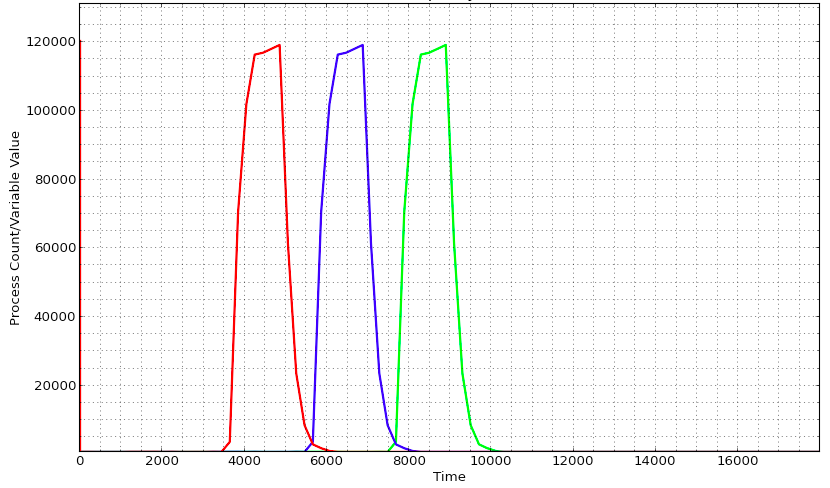
\includegraphics[width=0.8\textwidth]{images/asrc_graph_intro.png}
        \caption{Time Series Representation}
        \label{fig:asrc_graph_intro}
    \end{subfigure}
    \begin{subfigure}[b]{0.4\textwidth}
        \centering
        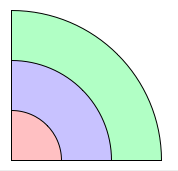
\includegraphics[width=0.5\textwidth]{images/asrc_cell_intro.png}
        \caption{Spatial Representation}
        \label{fig:asrc_cell_intro}
    \end{subfigure}
    \caption{One species at three locations in the cell represented traditionally on a time series graph and also spatially in a cell}
    \label{fig:asrc_intro}
\end{figure}


Over the course of the project the scope has been expanded.  The original objective was to assess which forms of visual representation are most helpful and informative to laboratory science.  At the end of the first project phase the objective changed (to reflect that the project was about delivering a finished program and not about the results of many experiments) to be to develop a tool to visualise the results of dynamic time-series models of intra-cellular behaviour based on biochemical reactions.  This objective was focused on visualisation to aid those researchers who are not numerically confident.  The second phase of the project has added to this objective to also aid interpretation and collaboration.  This change in objective is to make the tool better for all users.  To reflect these changes the focus on the original Src team has been generalised.  Evaluations are performed with other potential users who are also biologists.  Another factor in deciding to focus more on these other potential users was one of the key Src researchers going on maternity leave during the second phase of the project.  This made it infeasible to evaluate the tool with them.  It had been hoped to still evaluate the tool with them at the end of the second phase of development but they were still on maternity leave.

\section{Where Does This Tool Fit In?}
\label{sec:review}

In the first stage of the project a review was performed of the features of a number of modelling and visualisation tools.  This review included specialised software aimed at biologists and general software for anybody doing data visualisation.

As the project scope expanded to include goals not specifically related to visualisation it was prudent to perform another software review covering the new features, in particular software that allowed for collaborative editing.  It is important to see what features are commonplace, which features are not commonplace but are useful, and which features are not useful. This analysis would then be used to guide development of the collaborative features of the new tool.

Four products were chosen for this second review: Google Drive~\cite{g_drive}, Pidoco~\cite{pidoco}, Lucid Chart~\cite{lucid} and SynBiowave~\cite{sbw}.  Analysis of these software can be found below.

\subsection{Previously Reviewed Software}

The software packages reviewed at the start of the project were: Bio-PEPA, Uppaal~\cite{uppaal}, V-Cell~\cite{vcell}, Cell-O~\cite{cello}, Copasi~\cite{copasi}, Cell Designer~\cite{celldesigner} and WEAVE~\cite{weave}.  Bio-PEPA, V-Cell, Cell-O, Copasi and Cell Designer have been written for biological modelling.  Uppaal is modelling software for general use, and WEAVE is a general data visualisation tool.  A review of these tools can be find in MPP1 report for this project. \tdi{cite this?}

All offered some level of visualisation, some simply graphs, others more complex visualisations.  Bio-PEPA offered only line graphs.  Uppaal had visualisations that highlighted where in a finite state machine view of the model the current state is.  V-Cell had visualisation of the model in a hierarchical set of circles. It could also display spatial elements of the results data by displaying a heat model view of the cell.  Cell-O was aimed more at multi-cell models and was able to show them moving and splitting; it also had visualisation of the model as a finite state machine.  Copasi only had graphs, although the user had more control over the display of the plots.  WEAVE had the largest visualisation capacity being able to display a variety of standard graph types along with more interesting ones, such as geographical maps, but it did not appear to have anything specialised for biological models.  WEAVE is also the tool that gave the user the most control over the visualisation.

The existing biological modelling software seems to be focused more on the ease of modelling.  The visualisation features on offer are typically quite basic.  They also lack the more innovative features that can be found in the newer general data visualisation software.

\subsection{Google Drive}

Google Drive which was previously Google Docs, is one of the most widely used collaborative pieces of software.  Google Drive is used by a variety of user types.  The focus of the review was on the word processor.  Of the collaborative software reviewed this was felt to be the most user friendly.  One of the nicest features was a cursor indicating where every user currently editing the document is typing. Each user is also given a different colour allowing you to know who is doing what in real time.  Many people can edit a single document at once.  As well as editing documents users can also leave comments on the document.  Changes made by users appear near instantly to all users. The speed of editing is very important as it is frustrating as a user to have to wait to see changes others are making.  It is also very easy to invite others to edit the document with you.  Each document has a unique link and if a user visits that link they are taken to the document and can start editing.  Different permissions can be granted to different users allowing some level of collaboration with people who you don't necessarily want to grant full write access. These users can then just look at it in real time and offer comments.  Different parts of the editor have different levels of collaboration.  All text that is changed is changed for all, but preferences like font choice are only changed for the user, unless another user edits any text.  Also importantly from a \ac{UX} perspective is that any conflicts that arise appear to be resolved without any user intervention.  A history of what each user has done to the document is also provided and any unwanted changes can be rolled back.

\subsection{Pidoco}

Pidoco is a collaborative wireframing tool.  It was not as user friendly for collaboration as Google Drive.  Pidoco is much less instant.  Sometimes manual refreshes were required to display the work the other users had done.  Pidoco also supported multi user editing, however there was no way of seeing which users were editing a document. There was also a history of what changes each user had made.  Pidoco has no messaging or commenting system which makes asynchronous collaboration more difficult.  Sharing the work requires an email to be the sent to the user: they cannot simply be given a link.  Again different parts of the workspace have different levels of collaboration.  Any \ac{UI} widgets that are placed are shared, but if one user zooms in on a particular area other users are not forced to that zoom level.

\subsection{Lucid Chart}
Lucid Chart is a collaborative diagramming tool.  Lucid Chart lies between Google Drive and Pidoco in terms of collaboration speed.  It is not as instantaneous as Google Drive, but it does not require periodic manual refreshes like Pidoco.  It also allows multi user collaboration and documents can be shared by link or email.  Users can be granted read or read and write permissions on the document, like Google Drive, so you can collaborate with people you don't want to be able to fully edit.  It has a chat system and users can comment on the document making asynchronous collaboration easier.  Lucid Chart does not let you see what a user is doing in real time, but it does provide a full revision history so you can see what changes each user has made.  Lucid Chart is different in that it appears to be fully collaborative. Even font preferences are synced across users: if one user clicks bold all users will start typing in bold.

\subsection{SynBioWave}

SynBioWave was a biological extension to Google Wave.  It is the only example found of a platform for real time collaboration.  Unfortunately it could not be made to work.  The instruction page still refers to Google Wave.  Google Wave has been discontinued since 2012 (some of its real time features found their way into Google Docs).  An attempt was made to follow the instructions using Apache Wave (Google Wave was handed over to the Apache foundation) but the SynBioWave tool did not work.  The user guide does seem to give a good indication of how the tool would work.  The review is based on this.  Wave was used to enable the collaboration.  You would create a new wave and add your human collaborators.  You would also add the SynBioWave agent as a collaborator.   When the SynBioWave agent is added to the wave it adds a menu bar. Through this menu the human collaborators can call various functions; the agent then calculates the result and displays the visualisations.  The agent and its results can be interacted with in real time. SynBioWave is modular and there are multiple agents available.  Custom agents can also be created.  The use of Google Wave allowed the biologists to focus on implementing domain functionality without having to worry about the code infrastructure for real time collaboration.  Unfortunately, by relying on a third party for the backbone of the system, SynBioWave appears to have become unusable after Google Wave shut down.

\subsection{Findings}

From studying the alternative modelling tools available and their visualisation capabilities it was clear that the visualisation capabilities of Bio-PEPA had to be increased.  It was also clear that all the modelling tools were limited in their visualisation capability and that increasing the interactivity and customization available would be very useful.

We can see that there are a number of tools now that offer the ability to collaborate in real time.  Only one, however, could be found that was focused on synthetic biology.  This one tool appeared to now be obsolete.  Given how useful tools like collaborative document editors have been more commonplace it seems like a good idea to try and bring this functionality into the systems biology domain.  This would give Bio-PEPA a competitive advantage and hopefully encourage more researchers to use it.

\section{Previous Work}

Early on in the first stage of the project it was decided to separate this project from the Eclipse plug-in.  It was felt that Eclipse is not the right tool to do data visualisation in.

The initial development stages were focused on getting the new tool from having zero functionality to matching the visualisation features of the Eclipse plug-in.  This involved writing an early version of the \ac{UI}, parsing the Bio-PEPA results data, and plotting it using matplotlib~\cite{mpl}.

The next stage of the project was to extend the functionality.  The first new feature was intensity plotting where the colour of the line increases in intensity/opaqueness as the population of the species increases.  The next feature added was visualisation of the model.  Model visualisation used a system of nesting circles and rings to build a hierarchical view of the cell from its model components.  Finally the user was given control of the plot, allowing them to alter whether lines are plotted or not, what colour the line is and the thickness of the line.  Figure~\ref{fig:f75_mac_intro} shows how the main screen of the program looked at the end of the first stage of development (MPP1).

\begin{figure}[h!]
    \centering
    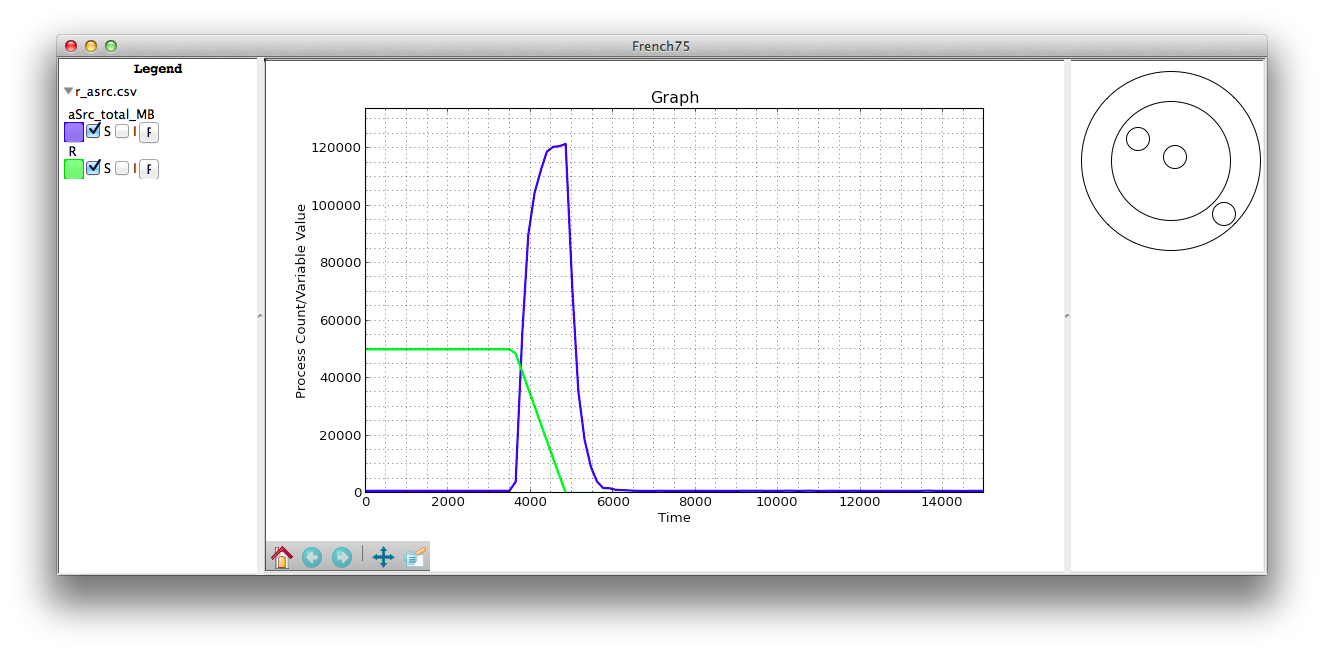
\includegraphics[width=\textwidth]{images/french75_mac.png}
    \caption{Main Screen of the Tool at the End of the First Stage of Development}
    \label{fig:f75_mac_intro}
\end{figure}

Over the course of the first stage of work a number of evaluations were carried out with potential and actual users of Bio-PEPA.  The findings from these evaluations were used to improve the tool.

\section{Results}
\tdi{should this go after libraries used?}

The tool that has been developed for this project is a fully featured tool with innovative features.  It has been positively received by potential users.
The tool offers more visualisation and analysis capabilities than the Eclipse plug-in.  Users can fully customize the appearance of the visualisation.  There is also the ability to add supporting information to the visualisation with annotations and the ability to attach files.  Sessions can be saved and loaded allowing users to spread their work over time.

There are also features aimed at making it easier for biologists who aren't comfortable analysing graphs to analyse their work.  This has been implemented as animated cell segments simulating the movement of species through the cell.

Innovative features include using plots as queries to find similar plots allowing for discoverability from within the tool, and real time collaboration that allows two collaborators to work together and see each others changes in real time.

Their is focus on ease of use in the finished product with all features made as easy as possible to use with little guidance.  Relying on recognition not recall.

By implementing more advanced visualisation features this tool should make Bio-PEPA a more attractive modelling tool. The visualisation features have been brought into line with the features in alternative modelling tools.

\subsection{This Document}

The rest of this document details the work that was undertaken during the second phase of this project (MPP2).  This is split into separate sections.

Chapter~\ref{chap:goals} discusses the goals that had been identified and the new goals that have been added.  This discussion includes what goals have been refined and why certain goals have been dropped.

Chapter~\ref{chap:work} discusses the implementation work that has been performed as part of this project phase.  The discussion includes challenges faced and solutions for those challenges.

Chapter~\ref{chap:eval} discuss the evaluation of the project.  This is spread over multiple evaluation sessions and includes evaluations with potential users as well as self evaluations.

\section{Libraries Used}

This section details the libraries that were used to build this project.  They are all Python libraries.  Some libraries have been more important than others.  This is detailed below.

\subsection{matplotlib}

matplotlib~\cite{mpl} is a graphing library for Python.  The graph visualisation is built on top of matplotlib.  The graph visualisation acts a wrapper around matplotlib.  The user does not have to write scripts that make calls to matplotlib.

Features built on top of matplotlib are:
\begin{itemize}
\item Intensity Gradient Plotting
\item Annotation infrastructure
\item Data normalisation
\item Line preferences
\end{itemize}

\subsection{wxPython}

wxPython~\cite{wxpython} is the \ac{GUI} library.  The \ac{GUI} and the animation visualisation are built on top of wxPython.  The animation visualisation uses wxPython's drawing api.  This is detailed further in Sections~\ref{sec:animation}~\&~\ref{sec:anime_annotation}

Features build on top of wxPython are:
\begin{itemize}
\item The \ac{UI}
\item Animation visualisation
\item Animation annotations
\end{itemize}

\subsection{SimpleXMLRPCServer}

SimpleXMLRPCServer~\cite{xmlrpcserver} has been used to enable communication between instances of the program.  SimpleXMLRPCServer was used to avoid having to write client and server code that would send and receive messages over sockets.  This allowed the development to focus on implementation of the \ac{API}

Built on top of this library is
\begin{itemize}
\item Real time collaboration
\end{itemize}

\subsection{Singleton}
\tdi{talk about the singleton}

\subsection{Miscellaneous}
A number of other Python libraries were utilised in the project.  They are all part of the standard Python library.  They did not provide any significant relevant behaviour, instead they were used to aid implementation of the features in this project.  More significant discussion of how any of these libraries were used can be found around the discussion of the features that utilised them.  The libraries are: uuid, re, platform, os, time, threading, subprocess, copy, random, numpy, itertools, collections, math, pickle, sys, inspect.

